\documentclass[conference]{IEEEtran}
\usepackage{amsmath,amssymb,amsfonts}
\usepackage{algpseudocode}
\usepackage{booktabs}
\usepackage{algorithm}
\usepackage{graphicx}
\usepackage{textcomp}
\usepackage{tikz}
\usepackage{xcolor}
\usepackage{multirow}
\usepackage[%
  backend=biber,
  urldate=iso,
  seconds=true,
  mincitenames=1,
  maxcitenames=3,
  minbibnames=1,
  maxbibnames=3,
  sorting=none,
]{biblatex}
\addbibresource{refs.bib}
\usetikzlibrary{positioning, chains, fit, arrows.meta, shapes}

\usepackage{listofitems}
\usepackage[outline]{contour}
\contourlength{1.4pt}

\usepackage{xcolor}
\colorlet{myred}{red!80!black}
\colorlet{myblue}{blue!80!black}
\colorlet{mygreen}{green!60!black}
\colorlet{myorange}{orange!70!red!60!black}
\colorlet{mydarkred}{red!30!black}
\colorlet{mydarkblue}{blue!40!black}
\colorlet{mydarkgreen}{green!30!black}

\tikzset{
  >=latex,
  node/.style={thick,circle,draw=myblue,minimum size=22,inner sep=0.5,outer sep=0.6},
  node in/.style={node,green!20!black,draw=mygreen!30!black,fill=mygreen!25},
  node hidden/.style={node,blue!20!black,draw=myblue!30!black,fill=myblue!20},
  node convol/.style={node,orange!20!black,draw=myorange!30!black,fill=myorange!20},
  node out/.style={node,red!20!black,draw=myred!30!black,fill=myred!20},
  connect/.style={thick,mydarkblue},
  connect arrow/.style={-{Latex[length=4,width=3.5]},thick,mydarkblue,shorten <=0.5,shorten >=1},
  node 1/.style={node in},
  node 2/.style={node hidden},
  node 3/.style={node out}
}
\def\nstyle{int(\lay<\Nnodlen?min(2,\lay):3)}

\DeclareMathOperator{\relu}{ReLU}
\newcommand{\empt}[2]{$#1^{\langle #2 \rangle}$}
\DeclareMathOperator{\sigmoid}{\sigma}
\DeclareMathOperator{\sigprime}{\sigma'}

\begin{document}

\title{Classification of Dry Beans}
\author{\IEEEauthorblockN{LG O'Donoghue \\ 18977995}
\IEEEauthorblockA{\textit{Department of Computer Science} \\
\textit{University of Stellenbosch}\\
Stellenbosch, South Africa \\
Email: 18977995@sun.ac.za}
}

\maketitle

\begin{abstract}
    Two machine-learning algorithms, K-Nearest Neighbours (KNN) and classification trees,
    are tasked with classifying a dry beans dataset. Data quality issues are discussed and
    accounted for with model-specific transformations. The models are implemented, calibrated, and
    compared. KNN is found to outperform classification trees slightly, but the classification tree
    implementation is preferred because the model requires significantly less data preprocessing.
\end{abstract}

\section{Introduction}

This report presents an analysis of the classification of dry beans using two different machine-learning approaches,
K-Nearest Neighbors (KNN) and Classification Trees.

First KNN and classification trees are introduced, followed by exploratory data analysis (EDA) of the dry beans
dataset.

Data quality issues are discovered and discussed. Transformations that address the data quality issues relevant
to the particular machine learning model are applied if necessary. The respective model control parameters are tuned,
on a training and validation set, with the final performance being evaluated on a test set.

In conclusion, the KNN model slightly outperforms the classification tree, but insignificantly so. The classification tree
is selected as the favourable model because of the minimal data preprocessing required compared to KNN.

The source code for this analysis can be found on \textbf{github.com/liam-od/DryBeans}.

\section{K-Nearest Neighbours}
KNN as discussed in \cite{fund}, is a non-parametric, supervised learning algorithm used for classification and regression tasks.
The algorithm uses inter-point distance measures to group points based on their closest neighbours. The general KNN algorithm is shown in Algorithm 1.

\begin{algorithm}
\caption{K-Nearest Neighbors (KNN) Classification}
\begin{algorithmic}[1]
    \Function{KNN}{$D$, $\mathbf{x}$, $k$}
    \For{all $\mathbf{x}_i \in D$}
        \State $\mathbf{d} = \textsc{Distance}(\mathbf{x}_i, \mathbf{x})$
    \EndFor
    \State \textsc{Sort}($\mathbf{d}$)
    \State $S \gets$ set of $k$ patterns in $D$ closest to $x$
    \State \Return majority class in $S$ \Comment{Ties are broken randomly}
\EndFunction
\end{algorithmic}
\end{algorithm}

\section{Classification trees}

Classification (or decision) trees are another supervised learning algorithm used for classification.
Classification trees are induced using a process of divide and conquer.
A training set, with $k$ classes, is recursively split into subsets of greater similarity until the classification tree overfits the training data \cite{fund}.
Algorithm 2 describes how the tree is induced.

\begin{algorithm}
\caption{Decision Tree Induction}
\begin{algorithmic}[1]
\Function{InduceTree}{$D$}
    \If{$|D| = 0$} \Comment{$D$ is empty}
        \State \Return leaf with default class
    \EndIf
    \If{$|D| > 0$ and $\forall x \in D$ the class is the same, i.e., $y_m$} \Comment{$D$ is homogeneous}
        \State \Return leaf with class label $y_m$, containing $D$
    \EndIf
    \Comment{$D$ is not homogeneous}
    \State Select a test based on a single input variable
    \State Split $D$ into $D_1, D_2, \ldots, D_O$, where $O$ is the number of outcomes
    \For{$o = 1$ to $O$}
        \State \textsc{InduceTree}($D_o$)
    \EndFor
\EndFunction
\end{algorithmic}
\end{algorithm}


\section{Characterization}

The characteristics of the features in the dry beans dataset are discussed in this section.
These characteristics are chosen because they enable the discussion of data quality issues within the dataset, as well as
provide insight into the meaning of the data.

\begin{table*}[htbp]
\centering
\caption{Data Summary}
\resizebox{\textwidth}{!}{%
\begin{tabular}{lrrrrrrrrrrrrrrrrr}
\toprule
Feature & dtype & encoded & cardinality & maj \% & na \% & na & q1 & q2 & q3 & mean & sd & min & max & skew & kurt & snr \\
\midrule
Area & Numeric & - & - & - & 0.0000 & - & 36328.0000 & 44652.0000 & 61332.0000 & 53048.2846 & 29324.0957 & 20420.0000 & 254616.0000 & 2.9529 & 10.8008 & 5.1493 \\
Perimeter & Numeric & - & - & - & 0.0000 & - & 703.5235 & 794.9410 & 977.2130 & 855.2835 & 214.2897 & 524.7360 & 1985.3700 & 1.6261 & 3.5881 & 12.0225 \\
MajorAxisLength & Numeric & - & - & - & 0.0000 & - & 253.3036 & 296.8834 & 376.4950 & 320.1419 & 85.6942 & 183.6012 & 738.8602 & 1.3578 & 2.5319 & 11.4481 \\
MinorAxisLength & Numeric & - & - & - & 0.0000 & - & 175.8482 & 192.4317 & 217.0317 & 202.2707 & 44.9701 & 122.5127 & 460.1985 & 2.2382 & 6.6511 & 13.0605 \\
AspectRation & Numeric & - & - & - & 0.0000 & - & 1.4323 & 1.5511 & 1.7071 & 1.5832 & 0.2467 & 1.0249 & 2.4303 & 0.5826 & 0.1138 & 16.1486 \\
Eccentricity & Numeric & - & - & - & 0.0000 & - & 0.7159 & 0.7644 & 0.8105 & 0.7509 & 0.0920 & 0.2190 & 0.9114 & -1.0628 & 1.3875 & 18.2360 \\
ConvexArea & Numeric & - & - & - & 0.0000 & - & 36714.5000 & 45178.0000 & 62294.0000 & 53765.6926 & 29778.0094 & -30.0000 & 263261.0000 & 2.9407 & 10.7397 & 5.1325 \\
Constantness & Numeric & - & - & - & 0.0000 & - & 1.0000 & 1.0000 & 1.0000 & 0.9029 & 0.2961 & 0.0000 & 1.0000 & -2.7212 & 5.4058 & 9.6829 \\
EquivDiameter & Numeric & - & - & - & 0.0000 & - & 215.0680 & 238.4380 & 279.4522 & 476.2541 & 25836.8656 & 0.1614 & 3014441.2390 & 116.6544 & 13609.1529 & -34.6877 \\
Colour & Categorical & no & 5 & 44.9269 & 0.0440 & ? & - & - & - & - & - & - & - & - & - & - \\
Extent & Categorical & no & 13530 & 0.0441 & 0.0441 & ? & - & - & - & - & - & - & - & - & - & - \\
Solidity & Numeric & - & - & - & 0.0000 & - & 0.9857 & 0.9883 & 0.9900 & 0.9871 & 0.0047 & 0.9192 & 0.9947 & -2.5501 & 12.7996 & 46.5195 \\
roundness & Numeric & - & - & - & 0.0000 & - & 0.8321 & 0.8832 & 0.9169 & 0.8733 & 0.0595 & 0.4896 & 0.9907 & -0.6357 & 0.3743 & 23.3302 \\
Compactness & Categorical & no & 13526 & 0.1322 & 0.1322 & ? & - & - & - & - & - & - & - & - & - & - \\
ShapeFactor1 & Numeric & - & - & - & 0.0000 & - & 0.0059 & 0.0066 & 0.0073 & 0.0066 & 0.0011 & 0.0028 & 0.0105 & -0.5341 & 0.7144 & 15.2970 \\
ShapeFactor2 & Numeric & - & - & - & 0.0000 & - & 0.0012 & 0.0017 & 0.0022 & 0.0017 & 0.0006 & 0.0006 & 0.0037 & 0.3012 & -0.8593 & 9.1873 \\
ShapeFactor3 & Numeric & - & - & - & 0.0000 & - & 0.5814 & 0.6420 & 0.6960 & 0.6436 & 0.0990 & 0.4103 & 0.9748 & 0.2425 & -0.1445 & 16.2601 \\
ShapeFactor4 & Numeric & - & - & - & 0.0000 & - & 1.6142 & 2.3688 & 3.1157 & 2.3681 & 0.8716 & 0.6956 & 3.9661 & 0.0076 & -1.1837 & 8.6818 \\
ShapeFactor5 & Numeric & - & - & - & 0.0000 & - & 0.9937 & 0.9964 & 0.9979 & 0.9951 & 0.0044 & 0.9477 & 0.9997 & -2.7595 & 13.0381 & 47.1547 \\
ShapeFactor6 & Categorical & no & 13607 & 0.0367 & 0.0367 & ? & - & - & - & - & - & - & - & - & - & - \\
Class & Categorical & no & 8 & 26.0231 & 0.1249 & ? & - & - & - & - & - & - & - & - & - & - \\
\bottomrule
\end{tabular}
}
\end{table*}

In Table 1, the characteristics of each of the features are shown. These characteristics are calculated based on the original dataset
without any transformations.

The characteristics are, \emph{dtype}, which is the data type of the feature, being either numeric or categorical. \emph{Encoded} suggested
whether or not the categorical data has been numerically encoded. \emph{Maj \%} represents the percentage of the data that the majority class controls,
this characteristic provides information regarding the class balance of the feature. \emph{Na \%} is the percentage of missing values for the feature and \emph{na}, is
the value that represents a missing data point (commonly `?' in Table 1). The first, second and third quartiles are \emph{q1}, \emph{q2} and \emph{q3} respectively. 
The mean, standard deviation, minimum value, and maximum value are \emph{mean}, \emph{sd}, \emph{min}, and \emph{max} respectively. The skewness of
the feature is \emph{skew} and the kurtosis is \emph{kurt}. Lastly, the signal-to-noise ratio that quantifies the stochastic noise based on signal strength is \emph{snr} \cite{snr}. 

\begin{table*}[htbp]
\centering
    \caption{Updated Data Summary}
\resizebox{\textwidth}{!}{%
\begin{tabular}{lrrrrrrrrrrrrrrrrr}
\toprule
Feature & dtype & encoded & cardinality & maj \% & na \% & na & q1 & q2 & q3 & mean & sd & min & max & skew & kurt & snr \\
\midrule
Constantness & Categorical & yes & 2 & 90.2873 & 0.0000 & - & - & - & - & - & - & - & - & - & - & - \\
Extent & Numeric & - & - & - & 0.0441 & nan & 0.7186 & 0.7599 & 0.7869 & 0.7497 & 0.0491 & 0.5553 & 0.8662 & -0.8961 & 0.6455 & 23.6796 \\
Compactness & Numeric & - & - & - & 0.1324 & nan & 0.7626 & 0.8013 & 0.8343 & 0.7999 & 0.0617 & 0.6406 & 0.9873 & 0.0371 & -0.2202 & 22.2574 \\
ShapeFactor6 & Numeric & - & - & - & 0.0368 & nan & 45.2588 & 88.7667 & 134.2730 & 89.3586 & 51.8386 & 0.0005 & 178.9850 & 0.0068 & -1.2013 & 4.7300 \\
\bottomrule
\end{tabular}
}
\end{table*}

Before the main data quality issues are discussed, four stand-out cases from Table 1 need to be addressed. The features `Extent', `Compactness', and `ShapeFactor6'
are all numerical features but are stored in a string format. Additionally, the feature `Constantness' is binary categorical but is stored as numeric as it
is already encoded. In Table 2, these features are converted and the appropriate statistics are shown.

\begin{figure*}
    \centering
    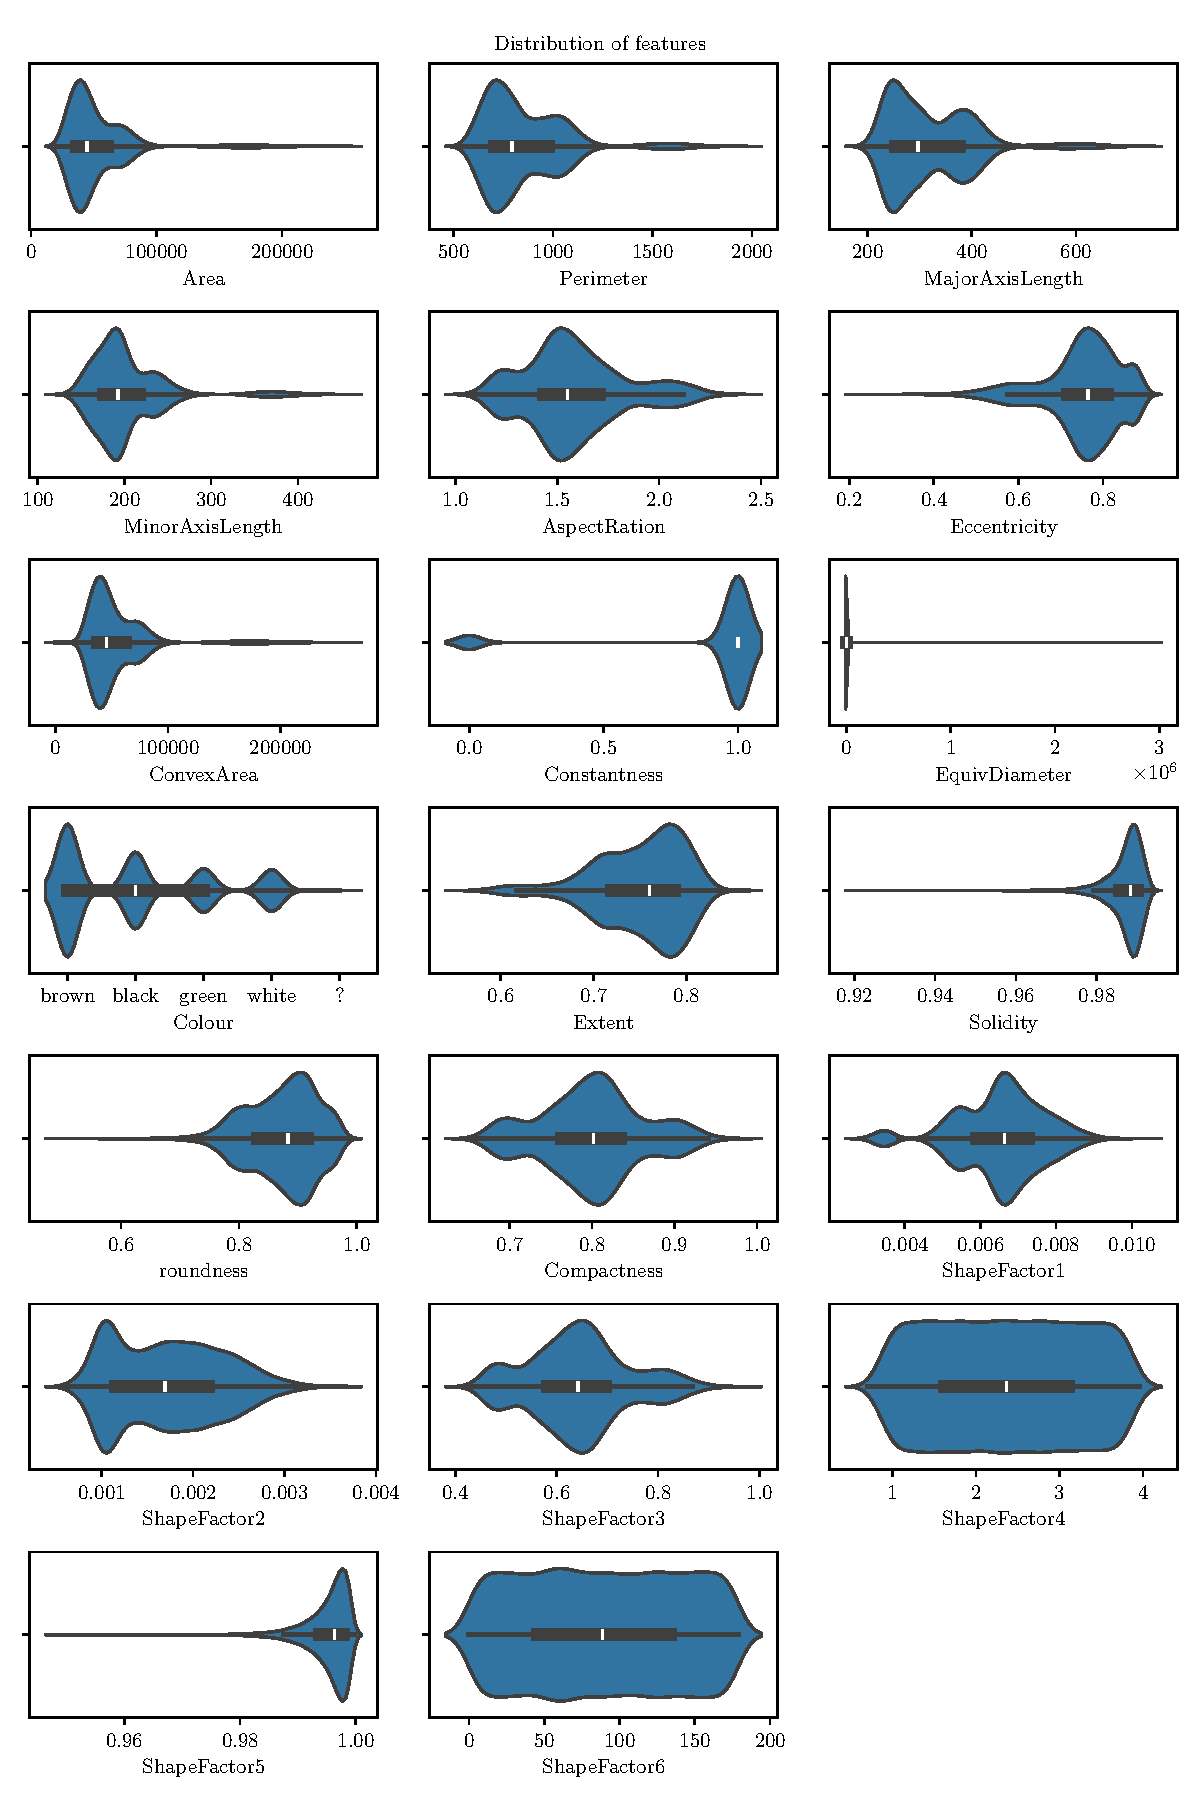
\includegraphics[scale=0.8]{test.pdf}
    \caption{Violin plots of features}
\end{figure*}

The violin plots in Figure 1, offer a means to better visualise the outliers and distribution of the features.

\section{Data quality issues}
The data quality issues that are exhibited by the features in the dry beans dataset are discussed in this section.
The data quality issues discussed are generic and not specific to any machine learning algorithm. The main
types of data quality issues that are focused on in this analysis are, missing values, outliers, noise, and skew or imbalanced data.

The features `Area', `Perimeter', `MajorAxisLength', `MinorAxisLength', `ConvexArea', and `EquivDiameter' all have large values with high standard deviations. Machine learning
models that are sensitive to the scale of the input features place more emphasis on features with a larger scale. This emphasis on the scale is undesirable as a feature with a smaller scale
might be more predictive than a feature with a larger scale \cite{fund}. Hence, these features are normalised using scikit-learns standard scaler \cite{sk}. Additionally, these features contain several outliers that are
significantly above the third quartile (or below the first quartile). These outliers stretch the scale of the data and distort statistical measures like the mean and standard deviation, which may
result in suboptimal learning \cite{fund}.

The `Extent', `Solidity', `roundness', `Compactness', and `ShapeFactor(1-5)' features, experience a similar scaling problem, but where the deviation in values is too small, which results in some machine learning
algorithms placing less emphasis on these features.

The `Colour', `Extent', `Compactness', `ShapeFactor6', and `Class' features all have missing values. Missing values can cause problems because they skew statistical measures and facilitate incomplete
training examples being provided to the machine learning model \cite{fund}. 

The signal-to-noise ratio indicates that the features `Area', `ConvexArea', `EquivDiameter', and `ShapeFactor6' contain varying degrees of noise, with `EquivDiameter` the worst case, possibly due to its extreme (probably invalid) outliers.
If the model is too complex, noise may lead to overfitting, where the noise is learned by the model. Some models perform better when noise is present \cite{fund}.

The `Constantness' feature has an imbalanced class distribution with $\approx 90\%$ of the data in the majority class. Skew or imbalanced features can result in high training accuracies for majority classes,
if the feature is the target feature in a classification problem.

Lastly, up until now, the outliers are assumed to be valid, however, the `ConvexArea' feature has a minimum value of $-30$, which seems like an invalid data entry.

\section{Preprocessing}
Now that the data quality issues are identified, the necessary preprocessing steps for each of the models of interest can be applied to the data.
First, for KNN, as discussed in section V, distance measures are sensitive to the scale of the data and outliers. Although KNN is generally robust to outliers concerning descriptive features,
because the outliers are not a nearest neighbour, standard scaling is applied to features with very high and very low standard deviations to mitigate the effect of emphasis being placed on features of a larger scale.
The invalid outliers are removed as they skew the features a lot, and then no more work is done to remove outliers, as both machine learning approaches are robust to outliers. Classification trees are robust to the scale of features because
of how the splitting mechanism uses relative ordering instead of absolute scale \cite{fund}. Hence, for the classification tree model, a standard scaler is not applied.

Although both models are sensitive to class imbalance, the `Constantness' feature is not transformed because it is not the target variable.

The missing values do not need to be imputed because their combined size is less than two percent of the data. This means that they can simply be removed from
the dataset. They are only removed for the KNN implementation as classification trees are robust to missing values because the algorithm treats missing values as
another category.

After the removal of the likely invalid outliers `EquivDiameter' is less noisy.
The other noisy features are not transformed because the noise is not in the target variable, where the KNN algorithm is most susceptible to noise \cite{fund}.

The remaining categorical features are now encoded with scikit-learns \emph{LabelEncoder} \cite{sk}, so that they can be used by the machine learning algorithms.

\section{The models}
The models are implemented using sklearn machine learning modules. The \emph{KNeighboursClassifier} for KNN, and
\emph{DecisionTreeClassifier} for the classification tree \cite{sk}.

First, a train test split is created where the training set is $80\%$ of the data, this ratio is ubiquitous in the literature and seems fitting for this use case.
Next, five-fold cross-validation is used to fit and evaluate the models. Five folds is also commonly used in the literature.
Several iterations of the training loop are run to calibrate the control parameters. The control parameter for KNN is \emph{n\_neighbours}, which is the number of
neighbouring points to consider, and the control parameters for the classification tree are \emph{max\_depth}, the maximum depth of the tree, and \emph{min\_samples\_split},
the minimum number of samples required to split at an internal node \cite{sk}.

Once the model is calibrated, a separate test set is used to evaluate the final model performance. The performance measure used is the f1 score, which is a commonly used
metric for classification tasks and it is a harmonic mean of precision and recall. The average of the f1 score for all classes is used as the final performance metric, this is known as the f1 macro score.
The f1 scores for each class are also considered individually to ensure that the model is not biased toward any particular class \cite{sk}.

\begin{figure}
    \centering
    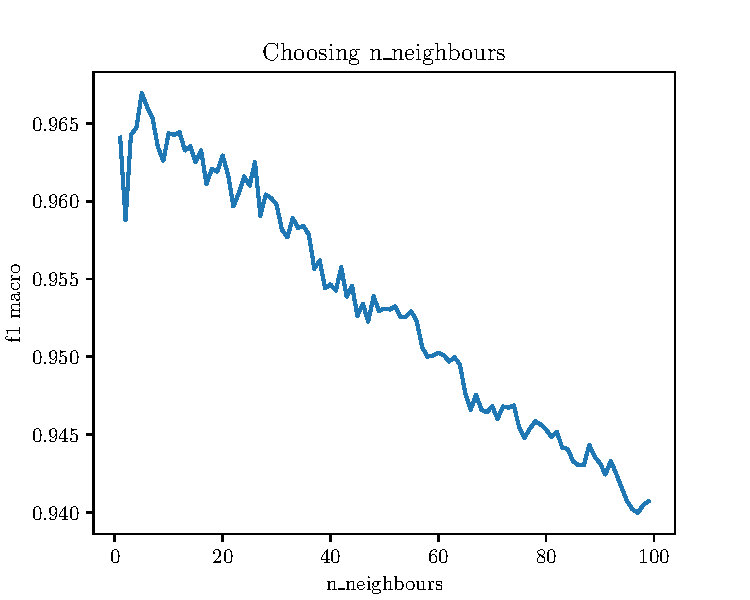
\includegraphics[scale=0.8]{neigh.pdf}
    \caption{Neighbours calibration}
\end{figure}

\begin{figure}
    \centering
    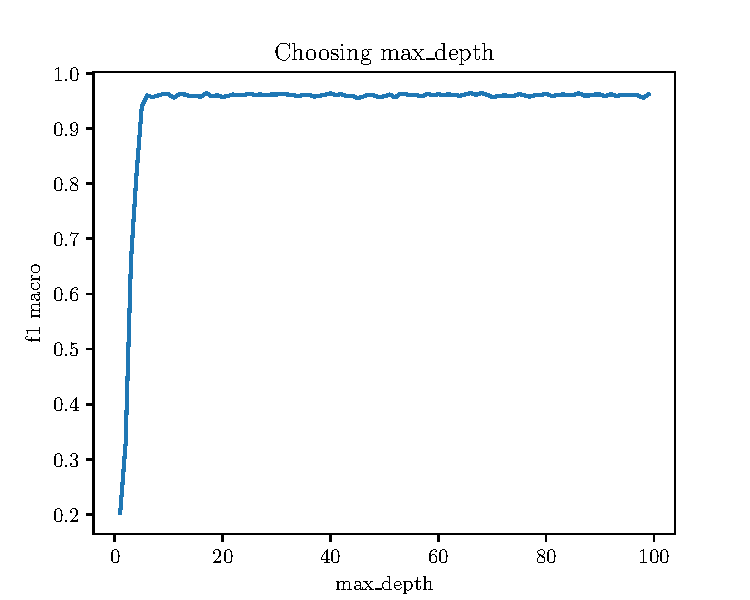
\includegraphics[scale=0.8]{depth.pdf}
    \caption{Max depth calibration}
\end{figure}

\begin{figure}
    \centering
    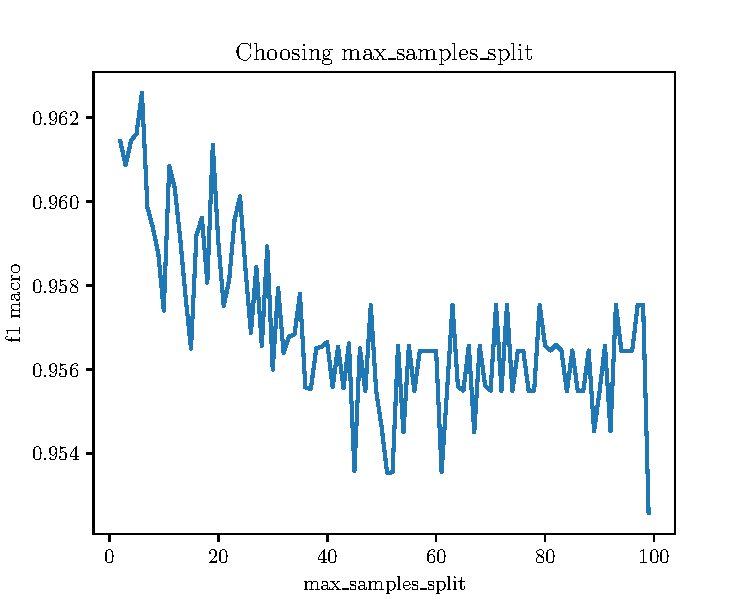
\includegraphics[scale=0.8]{samples.pdf}
    \caption{Min samples calibration}
\end{figure}

In Figure 2, the results of KNN calibration are shown, with \emph{n\_neighbours} $= 5$ being chosen. In Figures 3 and 4, the results of the classification tree calibration are shown, with \emph{max\_depth} $=6$ and
\emph{min\_samples\_split} $=5$.

Table 3, shows the average f1 macro scores for the five-fold cross-validation for each model, as well as the f1 macro scores for the test set.

\begin{table}[h]
    \centering
    \caption{Comparison of Classifier Performance}
    \begin{tabular}{lcc}
        \toprule
        Classifier & Cross-validation F1 macro & Test F1 macro \\
        \midrule
        KNeighboursClassifier & 0.964 & 0.98 \\
        DecisionTreeClassifier & 0.961 & 0.97\\
        \bottomrule
    \end{tabular}
\end{table}

\section{Conclusion}
This report discussed the K-Nearest Neighbours (KNN) and classification tree methods for classifying dry beans.
Data quality issues and suggested transformations were discussed and implemented.
In conclusion, it can be seen that both model implementations were able to successfully classify the dry beans dataset.
K-Nearest Neighbours (KNN) was able to slightly outperform the classification tree implementation. However, because
KNN required significantly more preprocessing of the data, the classification tree, is the favourable model.

\nocite{*}
\printbibliography

\end{document}
